\documentclass[a4paper, 11pt]{article}
\usepackage[utf8]{inputenc}
\usepackage{graphicx}
\usepackage{fancyvrb} 
\usepackage{siunitx}
\usepackage[table, xcdraw, svgnames]{xcolor}
\usepackage{listings, lstautogobble}
\usepackage{subfig}

\renewcommand{\figurename}{Figuur}

\setlength{\parskip}{0.5em}

\title{Sensornetwerk Proof of Concept v0.2}
\author{Groep 5}
\date{September 2019}
\pagenumbering{gobble}

\begin{document}

\maketitle
\clearpage
\pagenumbering{arabic}
\clearpage

\section{Inleiding}
Dit document beschrijft de software implementaties van groep 5 voor het vak "Sensornetwerk Ontwerp" aan de Hogeschool van Amsterdam.

Het doel van de opdracht is om een dynamisch netwerk van sensornodes te maken, waarbij in dit document de nadruk ligt op de algemene netwerkstructuur en de implementatie in MCU van de sensornodes. Hiervoor geldt over het algemeen dat het stuk software wat in dit document beschreven wordt gelijk is voor alle sensornodes. Tijdens de ontwikkeling van de individuele sensorimplementaties (vak "Sensormodule Ontwerp") kan de code afhankelijk per node worden aangepast. 

Het doel van dit document is om een 'proof of concept' te geven van de algemene netwerkstuctuur waar de sensornodes tijdens het vak "Sensormodule Ontwerp" gebruik van zullen maken.


\section{Algemene Node Programma}
Zoals besproken in de inleiding van dit document het grootste deel van de programma code voor de node MCU's gelijk. In dit hoofdstuk wordt deze code besproken. 

\subsection{Routing}
Het is belangrijk dat het sensornetwerk dynamisch is. Dit wil zeggen dat het het netwerk waarover de sensordata verstuurd wordt op ieder willekeurig moment kan veranderen. In de praktijk gebeurt dit wanneer de draadloze sensornodes van positie veranderen of uit gaan. 

Om een 'up to date' beeld te houden van de beschikbare nodes in het netwerk houdt iedere node een routing tabel bij. Deze tabel wordt opgesteld uit berichten die ontvangen worden van de directe buren van de node. In die berichten staat informatie over de directe buren van de nodes die de berichten sturen. 

%%%%%Moet nog aangevuld worden (Zie GLO)%%%%%%%
\subsection{Flowchart}
Om de algemene node-code inzichtelijk te maken is gebruik gemaakt van een flowchart. In figuur~\ref{fig:flowchart} is deze flowchart te zien.

\begin{figure}[!h]
	\centering	
	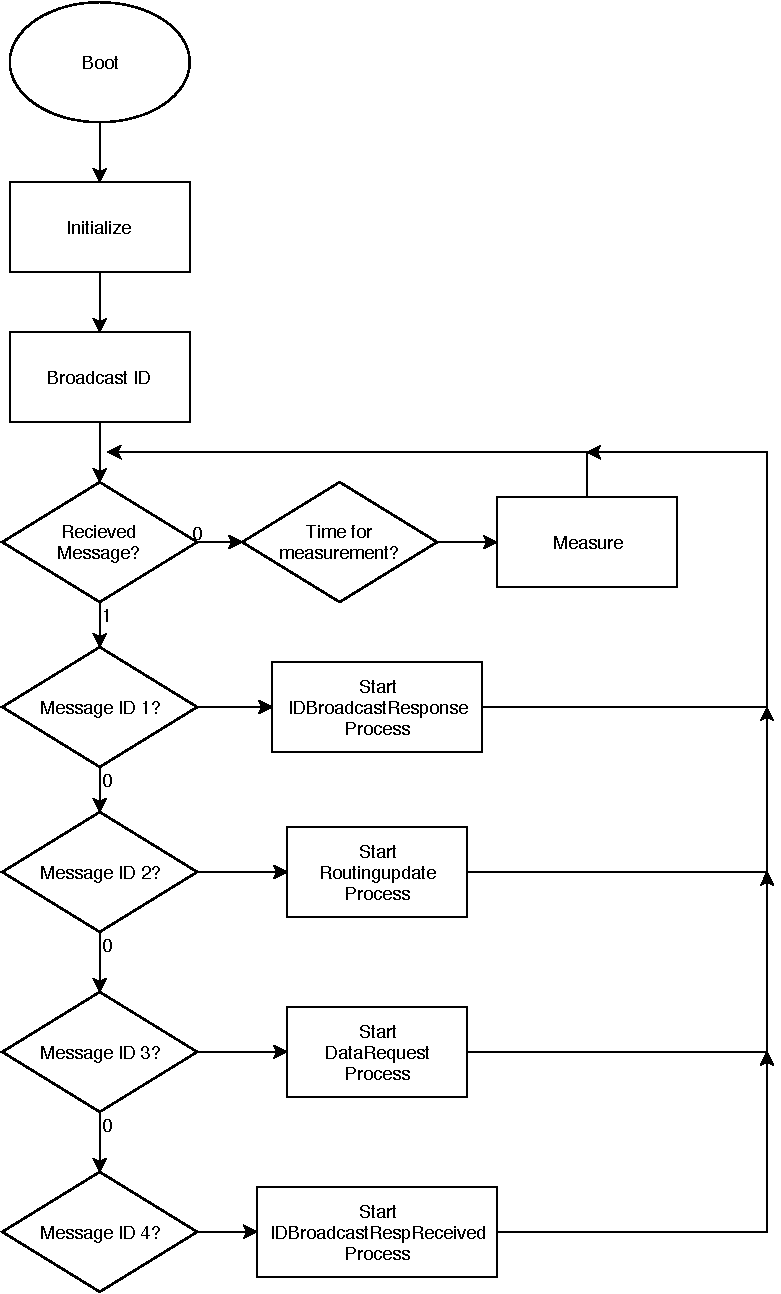
\includegraphics[width=.5\textwidth, keepaspectratio]{media/Pflow.pdf}
    \caption{Nadat de node opgestart is (Boot), wordt de MCU geïnitialiseerd in het blok [Initialize].\\
     \textbf{Figuur dient in deze versie als voorbeeld en zal geüpdatet worden wanneer het basisontwerp af is.}}
    \label{fig:flowchart}
\end{figure}
%Zie GLO

\subsection{Statemachine}
Een groot gedeelte van de tijd is de MCU is aan het wachten op berichten om deze vervolgens te verwerken. Daarom is er voor gekozen om een statemachine te gebruiken. Deze is afgebeeld in figuur~\ref{fig:Statemachine}.


\begin{figure}[!ht]
	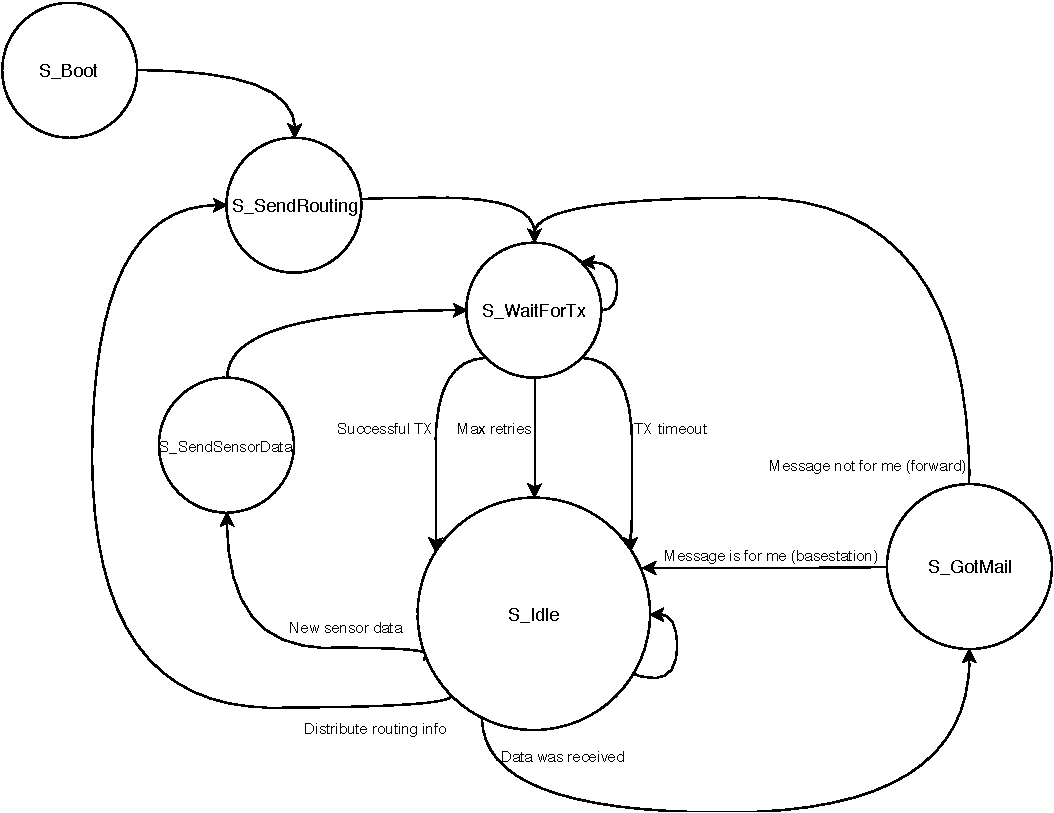
\includegraphics[width=.8\textwidth, keepaspectratio]{media/PState.pdf}
    \caption{Statemachine die de verschillende states laat zien waar de Xmega in komt vanaf het opstarten.\\ \textbf{Figuur dient in deze versie als voorbeeld en zal geupdate worden wanneer het basis ontwerp af is.}}
    \label{fig:Statemachine}
\end{figure}
%Zie GLO

\section{Basisstation}

\section{ISO groep}
Om te zorgen dat de nodes van de verschillende groepen elkaars datapaketten kunnen interpreteren en doorsturen zijn er afspraken gemaakt tussen de 5 groepen. Elke groep leverde 1 afgevaardigde, de 5 afgevaardigden vormden de ISO groep. De afspraken die de ISO-groep gemaakt heeft zijn opgesteld in\cite{ISO}. 

Naast afspraken over de algemene NRF-instellingen zijn er ook afspraken gemaakt over de berichttypes en de bijbehorende headers.

Bericht headers staan in de onderstaande tabel.

\subsection*{Message Types}
\begin{table}[!ht]
\begin{tabular}{|l|l|l|}
\hline
\rowcolor[HTML]{EFEFEF} 
Mask & Description           & Pipe \\ \hline
0x1  & ID Broadcast          & 0    \\ \hline
0x2  & Routine Routing Table & 1    \\ \hline
0x3  & Receive Port Data     & 1    \\ \hline
0x4  & Broadcast Reply       & 1    \\ \hline
\end{tabular}
\end{table}

\section{Netwerk Test}
Om te bewijzen dat het sensornetwerk waar de modules via zullen opereren werkt, zijn er verschillende tests uitgevoerd. Deze worden beschreven in onderstaande paragrafen.
\subsection{Routing Test}
TODO: Beschrijf een test voor het opzetten van een routing tabel met meerdere nodes.
\subsection{Basis Station test}
TODO: Beschrijf een test voor het testen van het Basisstation dat data ontvangt van meerdere nodes. 
\subsection{Demonstratie}
TODO: Beschrijf de demonstratie (oplevering blok 1).

\section{Demonstratie proof of concept} \label{demonstratie}
In dit hoofdstuk wordt beschreven hoe de "\textit{proof of concept}" gedemonstreerd wordt. Hierbij zal er onder andere uitleg worden gegeven over de test opstelling, situaties die invloed hebben op het netwerk (zoals het uitvallen van een node) en wat de verwachtingen zijn wanneer dergelijke situaties wel of niet optreden. Vervolgens wordt het netwerk onder deze omstandigheden getest en zal het vastgelegd worden d.m.v. datalogs. Op basis van deze datalogs zal uitgelegd worden of het gedrag van het netwerk overeen kwam met onze verwachtingen.
\newpage
\subsection{Testopstelling} \label{Testopstelling}
In figuur \ref{testopstelling} is de testopstelling te zien. Hierbij vertegenwoordigen 5 Xmega's de sensormodules en 1 Xmega het basisstation van het netwerk. De Xmega die het basisstation vertegenwoordigt is verbonden met een Raspberry Pi 3b+  waar een Raspberry 7 inch touchscreen display aan verbonden zit. Op dit display wordt alle ontvangen sensordata per sensormodule getoond en een routingtable waarin valt af te lezen welke nodes er zijn gezien in het netwerk en hoeveel hops deze verwijderd zijn van het basisstation.
\begin{figure}[h!]
	\centering
	%\hspace*{-2cm}
	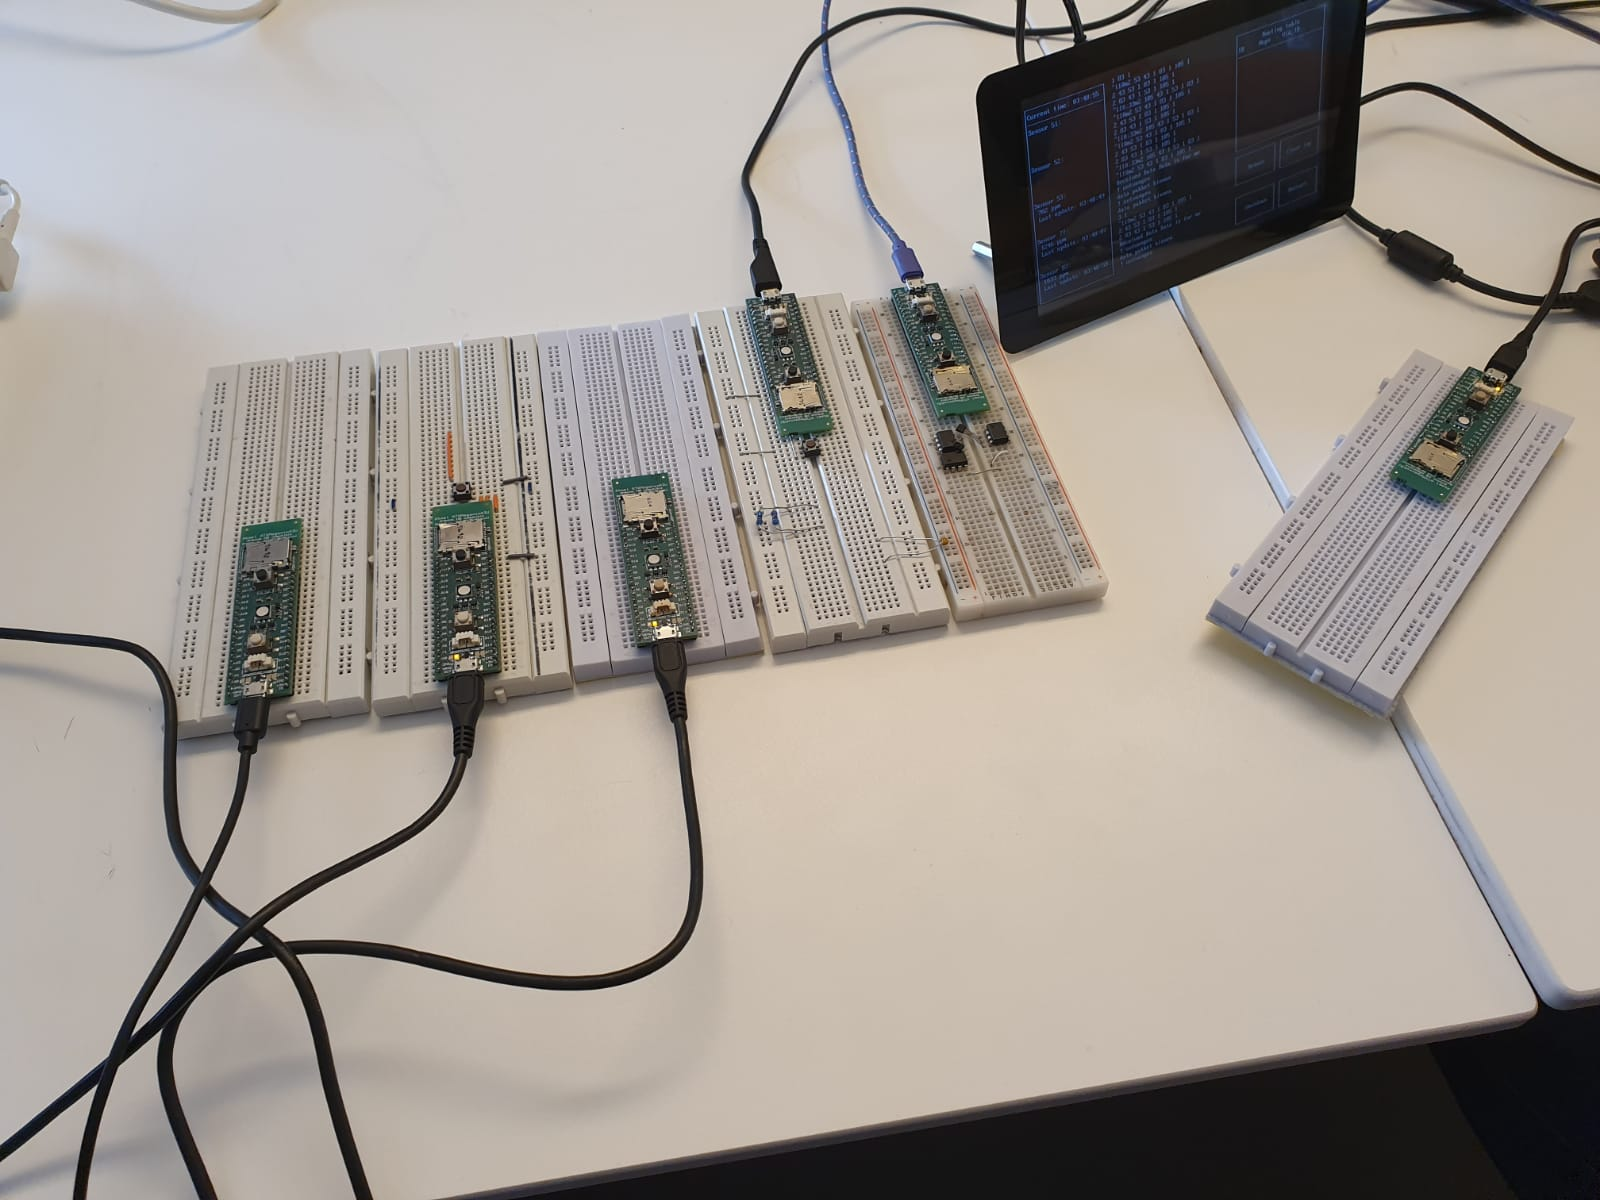
\includegraphics[width=8cm]{media/testOpstellingNetwerk.jpeg}
	\caption{Testopstelling voor de demonstratie van de proof of concept} \label{testopstelling}
\end{figure}

\newpage
\subsection{Situaties die het netwerk veranderen} \label{SituatieOmschrijving}
In tabel \ref{Situaties} is een overzicht te zien van alle situaties die een belangrijke invloed kunnen hebben op een node. Ook zal er in deze tabel worden omschreven wat de verwachtte reacties van het netwerk zijn op deze situaties.
\begin{table}[ht]
	\centering
	\caption{invloedrijke situaties voor het netwerk en de verwachtte reacties}
	\begin{tabular}{ | m{6cm} | m{6cm}| } 
		\hline
		\textbf{Situatie:} & \textbf{Verwachting:} \\
		\hline
		Sensormodule verplaatst zich richting een nieuwe buur & De verplaatste sensormodule zal aan de burenlijst worden toegevoegd van de buur waar hij zich naartoe verplaatst heeft
		\\
		\hline
		Sensormodule verplaatst zich van een buur af & De verplaatste sensormodule zal uit de burenlijst worden verwijderd van de buur waar hij zich vandaan verplaatst heeft en kan eventueel (afhankelijk van de richting en afstand) geen verbinding meer maken met andere sensormodules
		\\
		\hline
		Sensormodule valt opeens uit  & De sensormodule zal na een bepaalde tijd verwijderd worden uit de burenlijsten en zal in de routingtable bij het basis station als inactief worden gesteld
		\\ 
		\hline
		Sensormodule stuurt onzin data over het netwerk & Aangezien het deze berichten waarschijnlijk niet aan de ISO-standaarden voldoen zullen deze niet worden doorgestuurd of opgenomen door het basisstation
		\\ 
		\hline
		Signalen van een sensormodule worden opeens geblokkeerd & in principe hetzelfde als wanneer een sensormodule uitvalt. Verder zal de sensormodule na een bepaalde tijd alle buren uit de burenlijst verwijderen aangezien het ook geen berichten meer ontvangt
		\\ 
		\hline
		Sensormodule is niet direct verbonden met het basis station maar wel met andere sensormodules & De sensormodule zal proberen via andere sensormodules zijn data bij het basis station terecht te krijgen.
		\\
		\hline
	\end{tabular} 
	\label{Situaties}
\end{table}

\section{Demonstratie test}
In dit hoofdstuk worden de resultaten van de demonstratie test voor het proof of concept besproken. De demonstratie test is uitgevoerd volgens de testopstelling die wordt besproken in paragraaf \ref{Testopstelling} waarbij de diverse situaties die in paragraaf \ref{SituatieOmschrijving} getest worden. in tabel \ref{Situaties} is een overzicht te vinden van alle situaties die getest worden en wat de resultaten zijn die verwacht worden. De situaties zullen op volgorde van de tabel besproken worden.
\subsection{Sensormodule verplaats richting nieuwe buur} \label{VerplaatsNaar}
Om deze situatie te testen was er een sensormodule (met ID 52) op een dusdanige afstand van de andere modules geplaatst dat deze geen buren heeft, vervolgens is de sensormodule met ID 83 richting sensormodule 52 gelopen. De verwachting was dat sensormodule 83 zal worden toegevoegd aan de burenlijst van sensormodule 52.
\begin{figure}[h!]
	\centering
	%\hspace*{-2cm}
	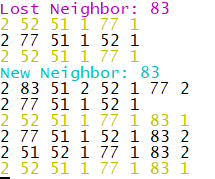
\includegraphics[width=4cm]{TestResults/LooptNaarNode/LoopNaarNieuweBuur_52_83.PNG}
	\caption{Nieuwe buur 83 wordt toegevoegd aan burenlijst} \label{LoopNaarNode}
\end{figure}
In figuur \ref{LoopNaarNode} is eerst te zien hoe sensormodule 83 uit de burenlijst verwijderd wordt omdat sensormodule 52 met een dusdanige afstand is verplaatst dat ze niet meer met elkaar in verbinding staan. Vervolgens verplaatst sensormodule 83 zich richting sensormodule 52, waarna er vervolgens in figuur \ref{LoopNaarNode} te zien is hoe deze weer wordt toegevoegd aan de burenlijst.

\subsection{Sensormodule verplaats van buur af}
Zoals bij de testsituatie van paragraaf \ref{VerplaatsNaar} wordt er bij deze testsituatie wederom gebruik gemaakt van sensormodules 52 en 83. Bij deze situatie zijn zowel sensormodule 52 als 83 beide op een dusdanige afstand van de andere sensormodules, dat ze alleen elkaar zien. Vervolgens verplaatst sensormodule 83 zich van 52 af. De verwachting is dat sensormodule 83 wordt verwijderd uit de burenlijst van 52.
\newpage

\begin{figure}[h!]
	\centering
	%\hspace*{-2cm}
	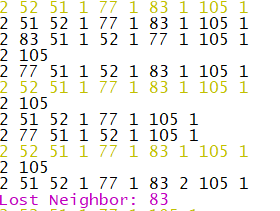
\includegraphics[width=4cm]{TestResults/LooptWegVanNode/LoopWegBijBuur_52_83.PNG}
	\caption{Buur 83 wordt verwijderd uit burenlijst} \label{LoopWegVanNode}
\end{figure}
In figuur \ref{LoopWegVanNode} is te zien hoe sensormodule 83 wordt verwijderd uit de burenlijst van sensormodule 52 nadat deze zo ver is verplaatst dat de verbinding verbroken werd.

\subsection{Sensormodule valt uit} \label{ValtUit}
Voor het testen van deze situatie waren alle nodes verbonden met elkaar. De debug log die is te zien in figuur \ref{NodeValtUit} is gegenereerd vanuit het basisstation. Uit het niets zal sensormodule 52 uitvallen omdat de voeding wordt afgesloten. De verwachting is dat het basisstation sensormodule 52 uit zijn burenlijst verwijderd.
\begin{figure}[h!]
	\centering
	%\hspace*{-2cm}
	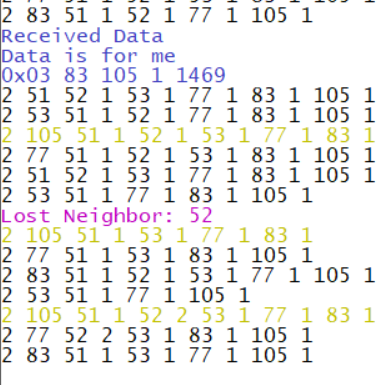
\includegraphics[width=4cm]{TestResults/NodeValtUit/NodeValtWeg_klein.png}
	\caption{Buur 52 wordt verwijderd uit burenlijst basisstation} \label{NodeValtUit}
\end{figure}
In figuur \ref{NodeValtUit} is te zien hoe het basisstation van alle 4 andere sensormodules (51, 53. 77, 83). Bij alle ontvangen berichten is de 2e byte het ID van de sensormodule, door te kijken van welk ID alle andere berichten komen is vast te stellen dat alle andere 4 sensormodules actief zijn. Uiteindelijk wordt sensormodule 52 verwijderd uit de burenlijst van het basisstation, omdat deze inactief is.

\subsection{Signalen sensormodule geblokkeerd}
Het testen van deze situatie was vergelijkbaar met die van paragraaf \ref{ValtUit}, echter i.p.v. dat sensormodule 52 van de voeding werd afgesloten, werd deze in een metalen kistje gestopt, zie figuur \ref{kistje}. 
\newpage
\begin{figure}[h!p]
	\centering
	%\hspace*{-2cm}
	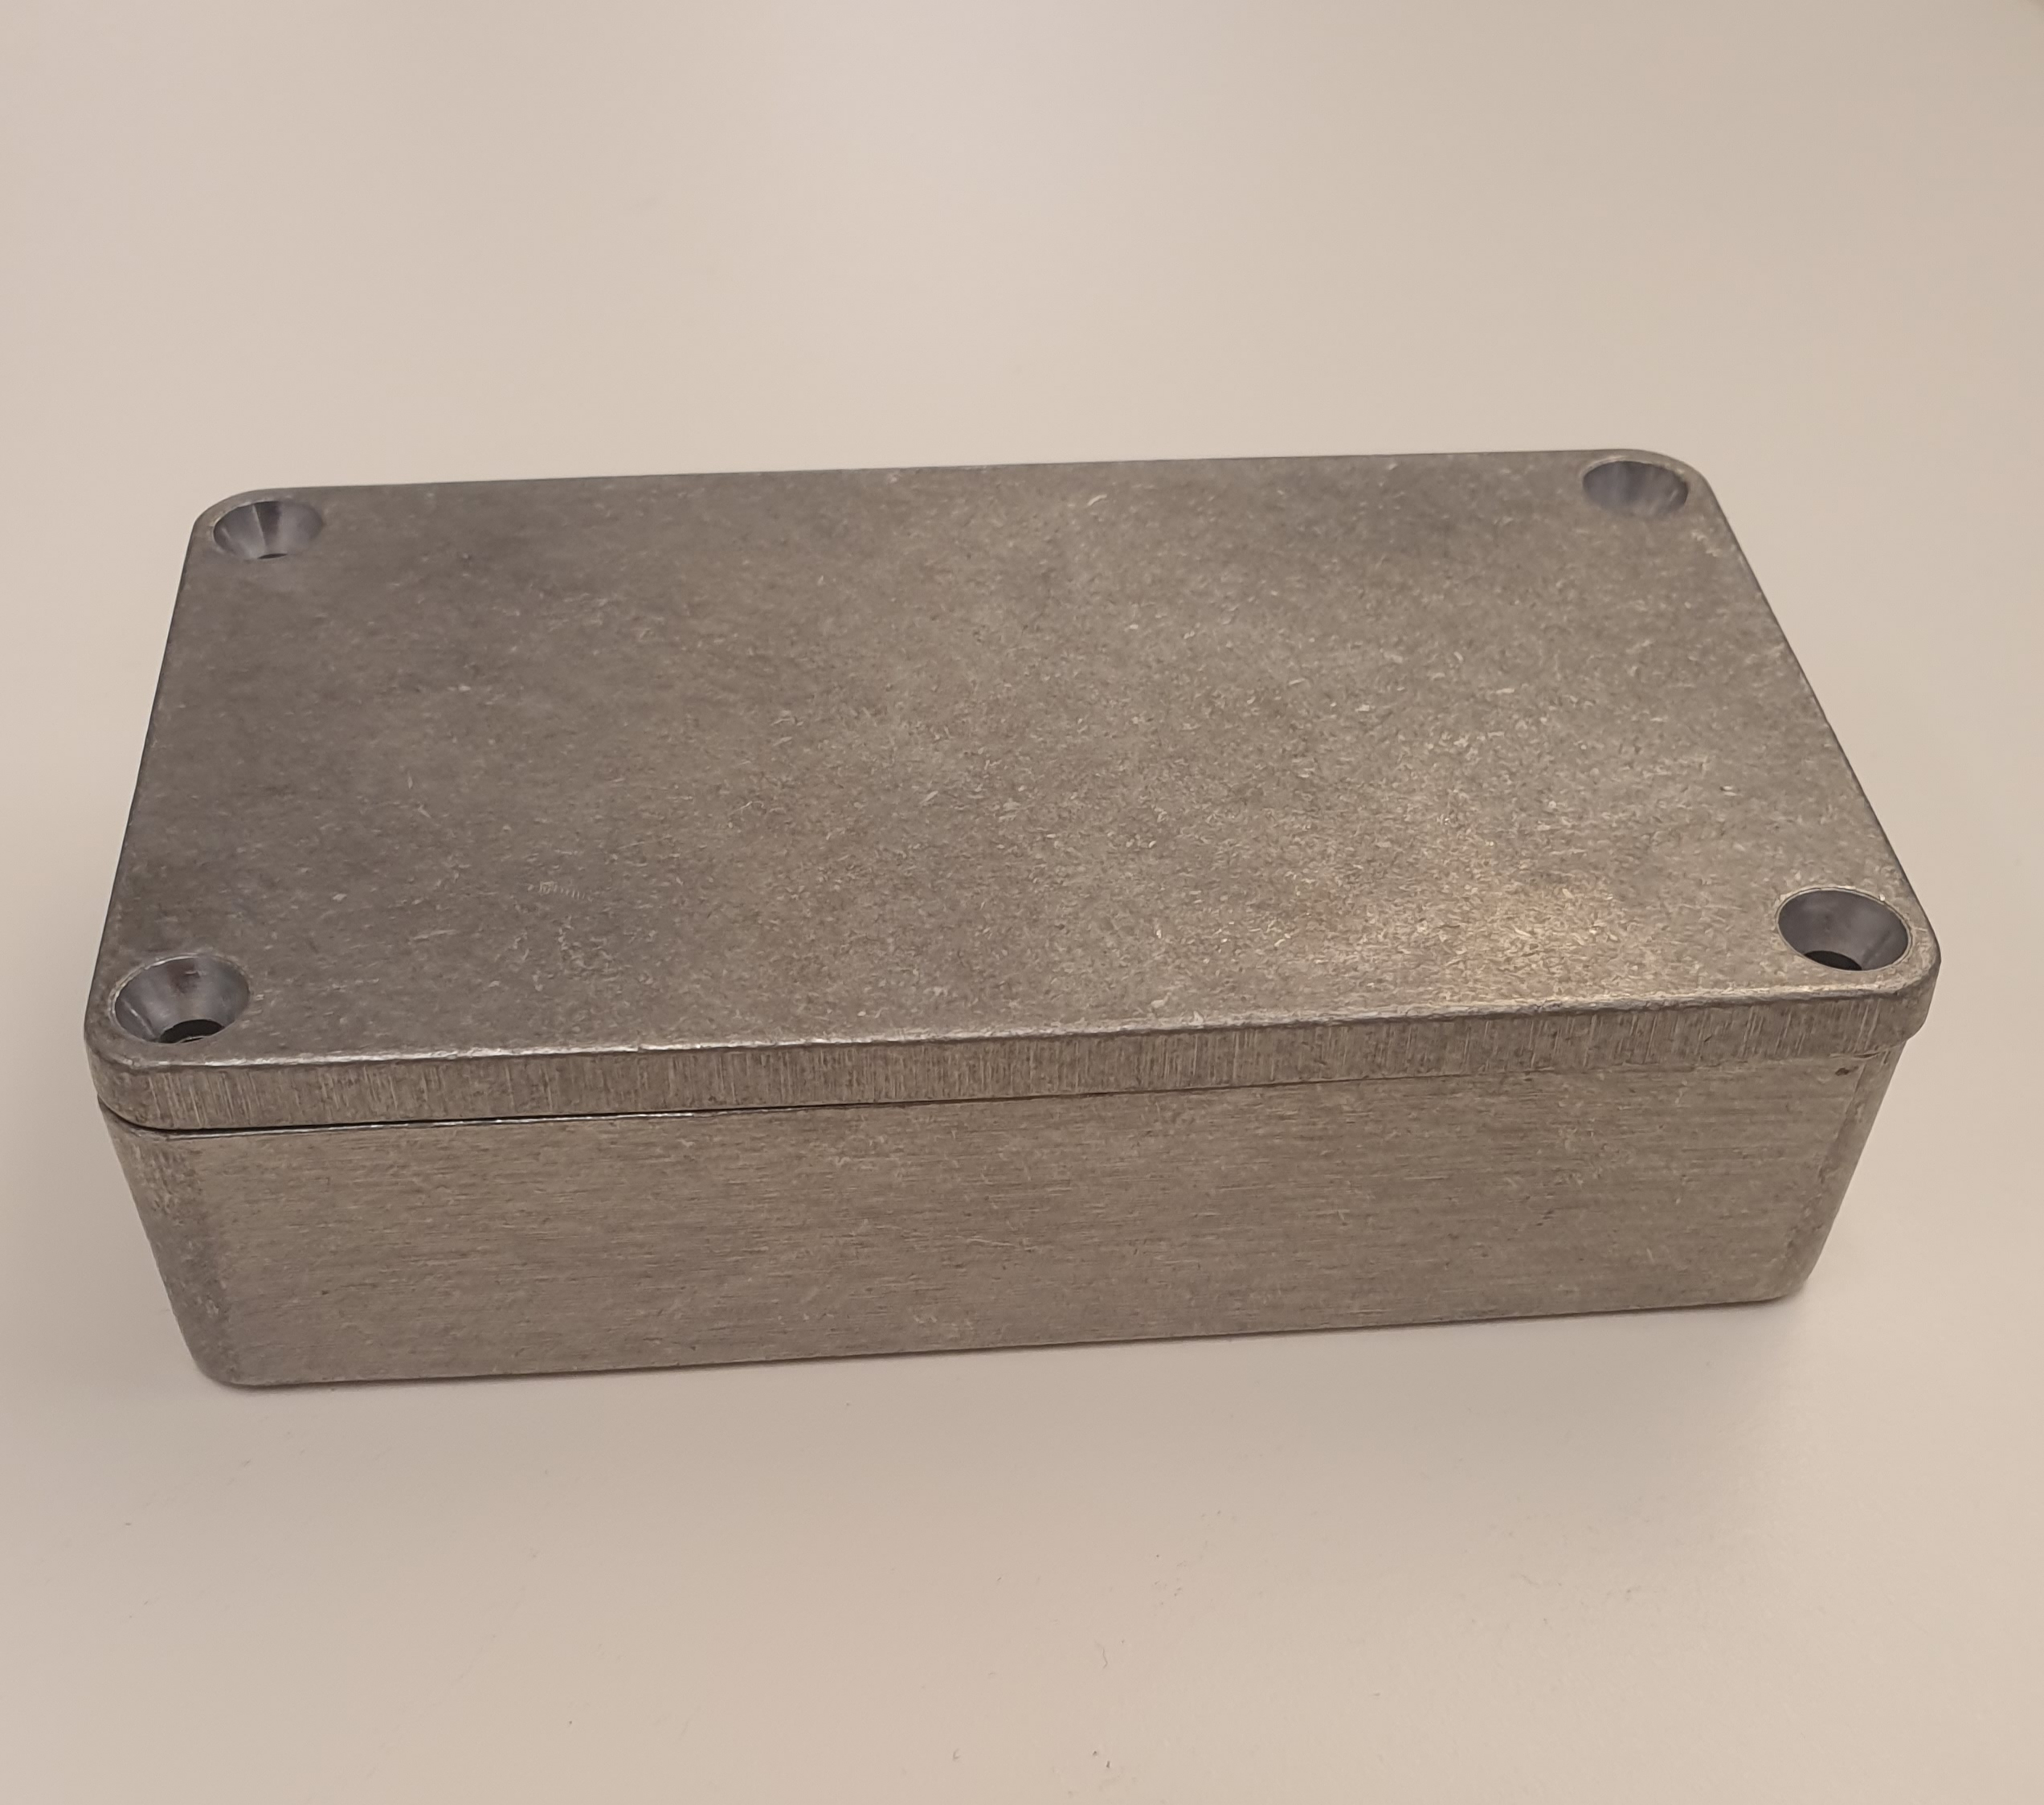
\includegraphics[width=4cm]{media/kistje.jpg}
	\caption{Metalen kistje voor signaal blokkade} \label{kistje}
\end{figure}
d.m.v. dit metalen kistje worden alle signalen van en naar sensormodule 52 geblokkeerd. De verwachting is dat sensormodule 52 wordt verwijderd uit de burenlijsten van alle andere sensormodules.
\begin{figure}[h!p]
	\centering
	%\hspace*{-2cm}
	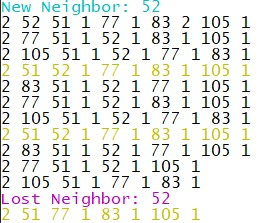
\includegraphics[width=4cm]{TestResults/FaradayKooi/51_Blokkade.jpeg}\hfill
	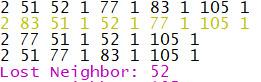
\includegraphics[width=4cm]{TestResults/FaradayKooi/83_Blokkade.jpeg}\hfill
	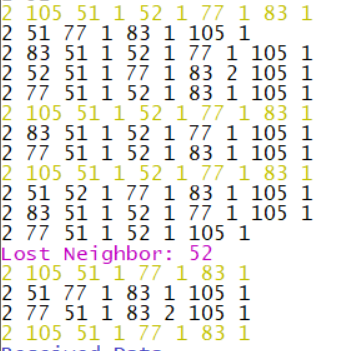
\includegraphics[width=4cm]{TestResults/FaradayKooi/105_verliest_52.png}
	\caption{sensormodule 51, 83 en het basisstation verwijderen 52 uit burenlijst} \label{faradayBlock}
\end{figure}
Zoals is te zien in figuur \ref{faradayBlock} wordt sensormodule 52 verwijderd bij de andere sensormodules. Wederom valt hier, net zoals in paragraaf \ref{ValtUit}, te zien hoe de andere sensormodules nog wel berichten ontvangen van elkaar.

\subsection{Data doorsturen via andere sensormodule}
Om deze situatie te testen is er een sensormodule op een bepaalde afstand van de rest van het netwerk gezet waardoor deze geen verbinding meer heeft met het netwerk. Vervolgens is er een andere sensormodule tussen het netwerk en het de "eenzame" sensormodule in geplaatst. De verwachting is dat de "eenzame" sensormodule verbinding maakt met sensormodule die er tussen is geplaatst, en via hem sensordata stuurt naar het basisstation. De "eenzame" sensormodule is 52, degene die er tussen is geplaatst is 83.
\newpage
\begin{figure}[h!]
	\centering
	%\hspace*{-2cm}
	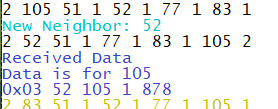
\includegraphics[width=5cm]{TestResults/DataViaBuur/83_StuurtDataDoor.jpeg}
	\caption{sensormodule 83 stuurt sensordata van 52 door} \label{Doorsturen83}
\end{figure}
In figuur \ref{Doorsturen83} is te zien hoe sensormodule 52 door 83 gezien wordt. Vervolgens ontvangt sensormodule 83 sensordata van 52, die voor het basisstation (105) bedoeld is (zie blauw bericht wat met 0x03 begint).
\begin{figure}[h!]
	\centering
	%\hspace*{-2cm}
	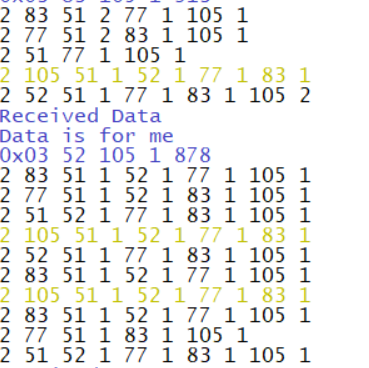
\includegraphics[width=5cm]{TestResults/DataViaBuur/DataRecevied105.png}
	\caption{basisstation ontvangt doorgestuurde data via 83} \label{Doorsturen105}
\end{figure}
In figuur \ref{Doorsturen105} is te zien hoe het basisstation de sensordata van sensormodule 52 ontvangt, terwijl het via sensormodule 83 is doorgestuurd. Zie hiervoor het blauwe bericht wat met 0x03 begint. Zoals bij alle andere berichten is de 2e byte het ID waar het bericht origineel vandaan komt, hieraan is te zien dat het bericht van sensormodule 52 komt. 
\newpage
\bibliographystyle{ieeetr}

\bibliography{POCbronnen} 

\end{document}